\chapter{Calculer des longueurs}
{https://sacado.xyz/qcm/parcours_show_course/0/117136}
{

\begin{His}
%\begin{wrapfigure}{l}{0.3\linewidth}
%\centering
%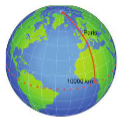
\includegraphics[width=\linewidth]{terre.PNG}
%\end{wrapfigure}
En $1790$, l'Assemblée nationale française décide d'établir un système de mesure unique. Il faut une mesure "pour tous les temps et pour tous les peuples". De nombreu.x.ses savant.e.s sont associé.e.s à ce projet. La Terre est alors choisie comme référence et le mètre défini comme la \textit{dix-millionième} partie du quart du méridien terrestre. \textbf{{\color{violet}Pierre Méchain}} ($1744-1804$) et \textbf{{\color{violet}Jean-Baptiste Delambre}} ($1749-1822$), astronomes et mathématiciens, déterminent une mesure précise de la longuer du méridien en $1798$. En $1799$, le mètre étalon est considéré comme définitif, il est déposé aux Archives nationales.

\vspace{0.3cm}
\textbf{{\color{violet}Archimède}} ($-287$,$-212$), mathématicien et ingénieur grec a déterminé une valeur approchée de $\pi$ en approchant le périmètre du cercle par le calcul des périmètres de polygones réguliers inscrits dans le cercle.

\begin{center}
\begin{tikzpicture}[line cap=round,line join=round,>=triangle 45,x=1.cm,y=1.cm]
\clip(-1.2896252389876417,-2.4335196421753236) rectangle (10.35430045927027,1.390666644471734);
\fill[line width=2.pt,color=zzttqq,fill=zzttqq,fill opacity=0.10000000149011612] (1.,0.) -- (-0.5,0.8660254037844386) -- (-0.5,-0.8660254037844388) -- cycle;
\fill[line width=2.pt,color=zzttqq,fill=zzttqq,fill opacity=0.10000000149011612] (4.,0.) -- (3.,1.) -- (2.,0.) -- (3.,-1.) -- cycle;
\fill[line width=2.pt,color=zzttqq,fill=zzttqq,fill opacity=0.10000000149011612] (10.,0.) -- (9.5,0.8660254037844387) -- (8.5,0.8660254037844386) -- (8.,0.) -- (8.5,-0.8660254037844386) -- (9.5,-0.866025403784439) -- cycle;
\fill[line width=2.pt,color=zzttqq,fill=zzttqq,fill opacity=0.10000000149011612] (7.,0.) -- (6.3090169943749475,0.9510565162951546) -- (5.190983005625052,0.5877852522924749) -- (5.190983005625051,-0.5877852522924725) -- (6.309016994374946,-0.9510565162951541) -- cycle;
\draw [line width=1.pt] (0.,0.) circle (1.cm);
\draw [line width=1.pt] (3.,0.) circle (1.cm);
\draw [line width=1.pt] (6.,0.) circle (1.cm);
\draw [line width=1.pt] (9.,0.) circle (1.cm);
\draw [line width=1.pt,color=zzttqq] (1.,0.)-- (-0.5,0.8660254037844386);
\draw [line width=1.pt,color=zzttqq] (-0.5,0.8660254037844386)-- (-0.5,-0.8660254037844388);
\draw [line width=1.pt,color=zzttqq] (-0.5,-0.8660254037844388)-- (1.,0.);
\draw [line width=1.pt,color=zzttqq] (4.,0.)-- (3.,1.);
\draw [line width=1.pt,color=zzttqq] (3.,1.)-- (2.,0.);
\draw [line width=1.pt,color=zzttqq] (2.,0.)-- (3.,-1.);
\draw [line width=1.pt,color=zzttqq] (3.,-1.)-- (4.,0.);
\draw [line width=1.pt,color=zzttqq] (10.,0.)-- (9.5,0.8660254037844387);
\draw [line width=1.pt,color=zzttqq] (9.5,0.8660254037844387)-- (8.5,0.8660254037844386);
\draw [line width=1.pt,color=zzttqq] (8.5,0.8660254037844386)-- (8.,0.);
\draw [line width=1.pt,color=zzttqq] (8.,0.)-- (8.5,-0.8660254037844386);
\draw [line width=1.pt,color=zzttqq] (8.5,-0.8660254037844386)-- (9.5,-0.866025403784439);
\draw [line width=1.pt,color=zzttqq] (9.5,-0.866025403784439)-- (10.,0.);
\draw [line width=1.pt,color=zzttqq] (7.,0.)-- (6.3090169943749475,0.9510565162951546);
\draw [line width=1.pt,color=zzttqq] (6.3090169943749475,0.9510565162951546)-- (5.190983005625052,0.5877852522924749);
\draw [line width=1.pt,color=zzttqq] (5.190983005625052,0.5877852522924749)-- (5.190983005625051,-0.5877852522924725);
\draw [line width=1.pt,color=zzttqq] (5.190983005625051,-0.5877852522924725)-- (6.309016994374946,-0.9510565162951541);
\draw [line width=1.pt,color=zzttqq] (6.309016994374946,-0.9510565162951541)-- (7.,0.);

\end{tikzpicture}
\end{center}
\end{His}
% \section{Les savoir-faire du parcours}

% \begin{CpsCol}
% \begin{itemize}
% \item Savoir mesurer la distance entre deux points.
% Savoir reporter une longueur.
% \item Savoir convertir des unités de longueurs.
% \item Savoir mesurer le périmètre d'un polygone.
% \item Savoir calculer le périmètre d'un polygone.
% \item Savoir calculer le périmètre de polygones particuliers avec une formule.
% \item Savoir utiliser la formule de calcul du périmètre d'un carré ou d'un rectangle.
% \item Savoir calculer la valeur axacte du périmètre d'un cercle.
% \item Savoir calculer une valeur approchée du périmètre d'un cercle.
% \end{itemize}
% \end{CpsCol}
}

\begin{pageCours} 

%\section{Mesurer et comparer des longueurs.}

\section{Le système métrique.}


\begin{Def}
Le \textbf{système métrique} est un \textbf{système décimal} :\\
\[1\, m=10\, dm \hspace{1cm} 1\, dm=10\, cm \hspace{1cm}1\, cm=10\, mm\]
\end{Def}

%\begin{Mt}
%On peut se servir d'un tableau de conversion.
%\begin{center}
%\begin{tabular}{c|c|c|c|c|c|c}
%    \textcolor{red}{kilo}mètre & \textcolor{red}{hecto}mètre & \textcolor{red}{déca}mètre & mètre & \textcolor{red}{déci}mètre & \textcolor{red}{centi}mètre & \textcolor{red}{milli}mètre  \\ \hline 
%    \textcolor{red}{k}m & \textcolor{red}{h}m & \textcolor{red}{da}m & m & \textcolor{red}{d}m & \textcolor{red}{c}m & \textcolor{red}{m}m \\ \hline
%    \(1 km = 1 000 m\) & \(1 hm = 100 m\) & \(1 dam = 10 m\) & \(1 m\) & \(1 dm = 0,1 m\) & \(1 cm = 0,01 m\) & \(1 mm = 0,001 m\)
%\end{tabular}
%\end{center}
%\end{Mt}


\begin{DefT}{Mètre}
L'\textbf{unité de longueur} est le \textbf{mètre}.\index{Mètre}
\end{DefT}



\begin{Mt}
On peut se servir d'un tableau de conversion.
\begin{center}
\begin{tabular}{|c|c|c|c|c|c|c|}\hline
%    \textcolor{red}{kilo}mètre & \textcolor{red}{hecto}mètre & \textcolor{red}{déca}mètre & mètre & \textcolor{red}{déci}mètre & \textcolor{red}{centi}mètre & \textcolor{red}{milli}mètre  \\ \hline 
    \textcolor{red}{k}m & \textcolor{red}{h}m & \textcolor{red}{da}m & m & \textcolor{red}{d}m & \textcolor{red}{c}m & \textcolor{red}{m}m \\ \hline
 &&&&&&  \\ \hline
%    \(1 km = 1 000 m\) & \(1 hm = 100 m\) & \(1 dam = 10 m\) & \(1 m\) & \(1 dm = 0,1 m\) & \(1 cm = 0,01 m\) & \(1 mm = 0,001 m\)
\end{tabular}
\end{center}
\end{Mt}

\section{Périmètre d'une figure.}

\begin{Ety}
Le mot {\color{orange}péri}{\color{violet} mètre} est composé du suffixe {\color{orange} péri} qui signifie le "\textit{autour de}" en grec et de sa racine {\color{violet} mètre} qui vient de mesure.   
\end{Ety}

\begin{DefT}{Périmètre}
Le périmètre\index{Périmètre} d'une figure est la longueur de son contour. L'unité de mesure du périmètre est le mètre.
\end{DefT}




\begin{Mt}
Pour calculer le périmètre d'un polygone, il suffit d'ajouter les longueurs de ses côtés exprimées \textbf{dans la même unité}.
\end{Mt}

\end{pageCours}
%%%%%%%%%%%%%%%%%%%%%%%%%%%%%%%%%%%%%%%%%%%%%%%%%%%%%%%%%%%%%%%%%%%%%%%%%%%%%%%%%%%%%%%%%%%%%%
%%%%%%%%%%%%%%%%%%%%%%%  Application directe
%%%%%%%%%%%%%%%%%%%%%%%%%%%%%%%%%%%%%%%%%%%%%%%%%%%%%%%%%%%%%%%%%%%%%%%%%%%%%%%%%%%%%%%%%%%%%%
\begin{pageAD} 

\ExoCad{Représenter.}

 Convertir les longueurs suivantes :
 
\begin{enumerate} 
\begin{minipage}{0.3\linewidth}\vspace{0.2cm}
\item $1 \,cm =  \ldots\ldots \,m$ \vspace{0.2cm}
\item $45 \,km =  \ldots\ldots\ldots\ldots \,cm$\vspace{0.2cm}
\item $100 \,mm =  \ldots\ldots \,dam$\vspace{0.2cm}
\end{minipage}
 \hfill
\begin{minipage}{0.3  \linewidth}
\item $1 20 \,cm =  \ldots\ldots \,dm$\vspace{0.2cm}
\item $4456 \,m =  \ldots\ldots \,km$\vspace{0.2cm}
\item $12 \,hm =  \ldots\ldots \,mm$\vspace{0.2cm}
\end{minipage}
 \hfill
\begin{minipage}{0.3  \linewidth}
\item $0,0033 \,km =  \ldots\ldots \,mm$\vspace{0.2cm}
\item $0,005 \,mm =  \ldots\ldots \,m$\vspace{0.2cm}
\item $1145 \,cm = \ldots\ldots \,m$\vspace{0.2cm}
\end{minipage}

\end{enumerate} 
 
 
\ExoCad{Représenter. Calculer.}
 
\begin{minipage}{.5\linewidth}
 
 Calculer le périmètre de la figure ABC en cm : 
\begin{tikzpicture}[line cap=round,line join=round,>=triangle 45,x=1.0cm,y=1.0cm]
\clip(1.,0.42) rectangle (6.32,3.54);
\draw [line width=1.pt] (5.42,2.92)-- (2.,1.);
\draw [line width=1.pt] (2.,1.)-- (4.,1.);
\draw [line width=1.pt] (5.42,2.92)-- (4.,1.);
\begin{scriptsize}
\draw [color=black] (5.42,2.92)-- ++(-2.5pt,0 pt) -- ++(5.0pt,0 pt) ++(-2.5pt,-2.5pt) -- ++(0 pt,5.0pt);
\draw[color=black] (5.56,3.29) node {$A$};
\draw [color=black] (2.,1.)-- ++(-2.5pt,0 pt) -- ++(5.0pt,0 pt) ++(-2.5pt,-2.5pt) -- ++(0 pt,5.0pt);
\draw[color=black] (1.44,1.21) node {$B$};
\draw[color=black] (3.6,2.41) node {$5,2~m$};
\draw [color=black] (4.,1.)-- ++(-2.5pt,0 pt) -- ++(5.0pt,0 pt) ++(-2.5pt,-2.5pt) -- ++(0 pt,5.0pt);
\draw[color=black] (4.24,0.99) node {$C$};
\draw[color=black] (3.06,0.85) node {$2,14~m$};
\draw[color=black] (5.24,1.89) node {$3,26~m$};
\end{scriptsize}
\end{tikzpicture}

\end{minipage} 
 \begin{minipage}{.5\linewidth}

\point{7} 
\end{minipage}
 
 
 
 
 

\ExoCad{Représenter. Calculer.}
 
 

 \begin{minipage}{.5\linewidth}
 
  Calculer le périmètre de la figure ci-dessous : 
  
 \begin{tikzpicture}[line cap=round,line join=round,x=1.0cm,y=1.0cm]
 \clip(-0.2806258071319262,-0.5469861082594564) rectangle (4.446308277251622,3.057396586133171);
 \draw [line width=1.pt,color=zzttqq] (0.,0.01527280802708741)-- (0.,2.5);
 \draw [line width=1.pt,color=zzttqq] (-0.045818424081262174,1.2285453939796842) -- (0.04581842408126196,1.2285453939796842);
 \draw [line width=1.pt,color=zzttqq] (-0.045818424081262174,1.2867274140474028) -- (0.04581842408126196,1.2867274140474028);
 \draw [line width=1.pt,color=zzttqq] (0.,2.5)-- (2.5,2.5);
 \draw [line width=1.pt,color=zzttqq] (1.2209089899661407,2.5458184240812622) -- (1.2209089899661407,2.4541815759187378);
 \draw [line width=1.pt] (1.279091010033859,2.5458184240812622) -- (1.279091010033859,2.4541815759187378);
 \draw [line width=1.pt,color=zzttqq] (2.5,2.5)-- (2.5,1.5);
 \draw [line width=1.pt,color=zzttqq] (2.5,1.5)-- (4.,1.5);
 \draw [line width=1.pt,color=zzttqq] (3.25,1.545818424081262) -- (3.25,1.4541815759187375);
 \draw [line width=1.pt,color=zzttqq] (4.,1.5)-- (4.,0.);
 \draw [line width=1.pt,color=zzttqq] (4.045818424081262,0.75) -- (3.9541815759187378,0.75);
 \draw [line width=1.pt,color=zzttqq] (4.,0.)-- (0.,0.01527280802708741);
 
 \draw [fill=ududff] (0.,0.01527280802708741) circle (2pt);
 \draw[color=ududff] (-0.028624474684984226,-0.3384384935348683) node {$A$};
 \draw [fill=ududff] (0.,2.5) circle (2pt);
 \draw[color=ududff] (-0.036260878698527926,2.7786678396388256) node {$B$};
 \draw [fill=ududff] (2.5,2.5) circle (2pt);
 \draw[color=ududff] (2.552480081892785,2.7557586275981945) node {$C$};
 \draw [fill=ududff] (2.5,1.5) circle (2pt);
 \draw[color=ududff] (2.3386607695135617,1.24302388509261) node {$D$};
 \draw [fill=ududff] (4.,1.5) circle (2pt);
 \draw[color=ududff] (4.056851672560893,1.9408436416208143) node {$E$};
 \draw [fill=ududff] (4.,0.) circle (2pt);
 \draw[color=ududff] (4.371397732764048,-0.06207445339943128) node {$F$};
 \draw[color=ududff] (1.0237457835361818,2.1899379827720288) node {$2.5\,cm$};
 \draw[color=ududff] (2.0928423454322995,2.0226638422979994) node {$1\,cm$};
 \draw[color=ududff] (3.22448363508463,1.14302388509261) node {$1.5\,cm$};
 \draw[color=ududff] (2.002658992917639,-0.2766205136025868) node {$4\,cm$};
 
 \end{tikzpicture}
\end{minipage} 
\begin{minipage}{.5\linewidth}

\point{7} 
\end{minipage}


\ExoCad{Communiquer.}

Trouver 3 mots avec le préfixe \textbf{péri} et donner leur définition.

\point{5}

\end{pageAD} 
 
%%%%%%%%%%%%%%%%%%%%%%%%%%%%%%%%%%%%%%%%%%%%%%%%%%%%%%%%%%%%%%%%%%%%%%%%%%%%%%%%%%%%%%%%%%%%%%
%%%%%%%%%%%%%%%%%%%%%%%  Cours
%%%%%%%%%%%%%%%%%%%%%%%%%%%%%%%%%%%%%%%%%%%%%%%%%%%%%%%%%%%%%%%%%%%%%%%%%%%%%%%%%%%%%%%%%%%%%%
\begin{pageCours} 






\section{Périmètre de polygones particuliers.}

\begin{Pp}
Le périmètre d'un triangle équilatéral est proportionnel à la longueur de ses côtés : $\mathcal{P}=3\times \textcolor{zzttqq}{c}$
\begin{center}
\begin{tikzpicture}[line cap=round,line join=round,>=triangle 45,x=0.6cm,y=0.6cm]
\clip(0.36,-2.49) rectangle (10.78,2.19);
\fill[line width=1.pt,color=zzttqq,fill=zzttqq,fill opacity=0.10000000149011612] (4.,-1.) -- (7.,-1.) -- (5.5,1.598076211353316) -- cycle;
\draw [line width=1.pt,color=zzttqq] (4.,-1.)-- (7.,-1.);
\draw [line width=1.pt,color=zzttqq] (5.45,-0.88) -- (5.45,-1.12);
\draw [line width=1.pt,color=zzttqq] (5.55,-0.88) -- (5.55,-1.12);
\draw [line width=1.pt,color=zzttqq] (7.,-1.)-- (5.5,1.598076211353316);
\draw [line width=1.pt,color=zzttqq] (6.171076951545868,0.1957368354874359) -- (6.378923048454133,0.31573683548743586);
\draw [line width=1.pt,color=zzttqq] (6.121076951545867,0.28233937586588015) -- (6.328923048454133,0.40233937586588014);
\draw [line width=1.pt,color=zzttqq] (5.5,1.598076211353316)-- (4.,-1.);
\draw [line width=1.pt,color=zzttqq] (4.8789230484541335,0.28233937586588015) -- (4.671076951545869,0.40233937586588014);
\draw [line width=1.pt,color=zzttqq] (4.828923048454134,0.1957368354874359) -- (4.621076951545869,0.31573683548743586);
\draw [line width=1.pt,color=zzttqq] (1.,-2.)-- (4.,-2.);
\draw [line width=1.pt,color=zzttqq] (2.45,-1.88) -- (2.45,-2.12);
\draw [line width=1.pt,color=zzttqq] (2.55,-1.88) -- (2.55,-2.12);
\draw [line width=1.pt,color=zzttqq] (4.,-2.)-- (7.,-2.);
\draw [line width=1.pt,color=zzttqq] (5.45,-1.88) -- (5.45,-2.12);
\draw [line width=1.pt,color=zzttqq] (5.55,-1.88) -- (5.55,-2.12);
\draw [line width=1.pt,color=zzttqq] (7.,-2.)-- (10.,-2.);
\draw [line width=1.pt,color=zzttqq] (8.45,-1.88) -- (8.45,-2.12);
\draw [line width=1.pt,color=zzttqq] (8.55,-1.88) -- (8.55,-2.12);
%\begin{scriptsize}
\draw [fill=ududff] (4.,-1.) circle (2pt);
\draw[color=ududff] (3.74,-0.52) node {$A$};
\draw [fill=ududff] (7.,-1.) circle (2pt);
\draw[color=ududff] (7.14,-0.54) node {$B$};
\draw [fill=ududff] (5.5,1.598076211353316) circle (2pt);
\draw[color=ududff] (5.64,1.96) node {$C$};
\draw [fill=ududff] (1.,-2.) circle (2pt);
\draw [fill=ududff] (4.,-2.) circle (2pt);
\draw [fill=ududff] (7.,-2.) circle (2pt);
\draw[color=zzttqq] (5.55,-1.4) node {$c$};
\draw [fill=ududff] (10.,-2.) circle (2pt);
%\end{scriptsize}
\end{tikzpicture}
\end{center}
\end{Pp}

\begin{Pp}

\begin{minipage}{0.4\linewidth}
Le périmètre d'un carré est proportionnel à la longueur de ses côtés : $\mathcal{P}=4\times \textcolor{zzttqq}{c}$
\end{minipage}
\begin{minipage}{0.4\linewidth}
\begin{tikzpicture}[line cap=round,line join=round,>=triangle 45,x=0.6cm,y=0.6cm]
\clip(-1.32,-2.57) rectangle (12.68,2.51);
\fill[line width=1.pt,color=zzttqq,fill=zzttqq,fill opacity=0.10000000149011612] (4.,-1.) -- (7.,-1.) -- (7.,2.) -- (4.,2.) -- cycle;
\draw [line width=1.pt,color=zzttqq] (-0.5,-2.01)-- (2.5,-2.01);
\draw [line width=1.pt,color=zzttqq] (0.95,-1.89) -- (0.95,-2.13);
\draw [line width=1.pt,color=zzttqq] (1.05,-1.89) -- (1.05,-2.13);
\draw [line width=1.pt,color=zzttqq] (2.5,-2.01)-- (5.5,-2.01);
\draw [line width=1.pt,color=zzttqq] (3.95,-1.89) -- (3.95,-2.13);
\draw [line width=1.pt,color=zzttqq] (4.05,-1.89) -- (4.05,-2.13);
\draw [line width=1.pt,color=zzttqq] (5.5,-2.01)-- (8.5,-2.01);
\draw [line width=1.pt,color=zzttqq] (6.95,-1.89) -- (6.95,-2.13);
\draw [line width=1.pt,color=zzttqq] (7.05,-1.89) -- (7.05,-2.13);
\draw [line width=1.pt,color=zzttqq] (4.,-1.)-- (7.,-1.);
\draw [line width=1.pt,color=zzttqq] (5.45,-0.88) -- (5.45,-1.12);
\draw [line width=1.pt,color=zzttqq] (5.55,-0.88) -- (5.55,-1.12);
\draw [line width=1.pt,color=zzttqq] (7.,-1.)-- (7.,2.);
\draw [line width=1.pt,color=zzttqq] (6.88,0.45) -- (7.12,0.45);
\draw [line width=1.pt,color=zzttqq] (6.88,0.55) -- (7.12,0.55);
\draw [line width=1.pt,color=zzttqq] (7.,2.)-- (4.,2.);
\draw [line width=1.pt,color=zzttqq] (5.55,1.88) -- (5.55,2.12);
\draw [line width=1.pt,color=zzttqq] (5.45,1.88) -- (5.45,2.12);
\draw [line width=1.pt,color=zzttqq] (4.,2.)-- (4.,-1.);
\draw [line width=1.pt,color=zzttqq] (4.12,0.55) -- (3.88,0.55);
\draw [line width=1.pt,color=zzttqq] (4.12,0.45) -- (3.88,0.45);
\draw [line width=1.pt,color=zzttqq] (8.5,-2.01)-- (11.5,-2.01);
\draw [line width=1.pt,color=zzttqq] (9.95,-1.89) -- (9.95,-2.13);
\draw [line width=1.pt,color=zzttqq] (10.05,-1.89) -- (10.05,-2.13);

\draw [fill=ududff] (4.,-1.) circle (2pt);
\draw[color=ududff] (3.44,-0.68) node {$A$};
\draw [fill=ududff] (7.,-1.) circle (2pt);
\draw[color=ududff] (7.4,-0.7) node {$B$};
\draw [fill=ududff] (-0.5,-2.01) circle (2pt);
\draw [fill=ududff] (2.5,-2.01) circle (2pt);
\draw [fill=ududff] (5.5,-2.01) circle (2pt);
\draw[color=zzttqq] (5.55,-1.4) node {$c$};
\draw [fill=ududff] (8.5,-2.01) circle (2pt);
\draw [fill=ududff] (7.,2.) circle (2pt);
\draw[color=ududff] (7.38,2.05) node {$C$};
\draw [fill=ududff] (4.,2.) circle (2pt);
\draw[color=ududff] (3.36,2.05) node {$D$};
\draw [fill=ududff] (11.5,-2.01) circle (2pt);
\end{tikzpicture}
\end{minipage}
\end{Pp}

\begin{Pp}

Le périmètre d'un rectangle de largeur $\textcolor{zzttqq}{l}$ et de longueur $\textcolor{zzttqq}{L}$ est :

\begin{minipage}{0.3\linewidth}

$\mathcal{P}=2\times(\textcolor{zzttqq}{l}+\textcolor{zzttqq}{L})$
\vspace{0.3cm}
$\mathcal{P}=2\times\textcolor{zzttqq}{l}+2\times \textcolor{zzttqq}{L}$
\end{minipage}
\begin{minipage}{0.7\linewidth}


\begin{tikzpicture}[line cap=round,line join=round,>=triangle 45,x=0.5cm,y=0.5cm]
\clip(-3.88,-5.63) rectangle (14.22,2.97);
\fill[line width=2.pt,color=zzttqq,fill=zzttqq,fill opacity=0.10000000149011612] (2.,-1.) -- (7.,-1.) -- (7.,2.) -- (2.,2.) -- cycle;
\draw [line width=1.pt,color=zzttqq] (2.,-1.)-- (7.,-1.);
\draw [line width=1.pt,color=zzttqq] (4.45,-0.88) -- (4.45,-1.12);
\draw [line width=1.pt,color=zzttqq] (4.55,-0.88) -- (4.55,-1.12);
\draw [line width=1.pt,color=zzttqq] (7.,-1.)-- (7.,2.);
\draw [line width=1.pt,color=zzttqq] (6.76,0.5) -- (7.24,0.5);
\draw [line width=1.pt,color=zzttqq] (7.,2.)-- (2.,2.);
\draw [line width=1.pt,color=zzttqq] (4.55,1.88) -- (4.55,2.12);
\draw [line width=1.pt,color=zzttqq] (4.45,1.88) -- (4.45,2.12);
\draw [line width=1.pt,color=zzttqq] (2.,2.)-- (2.,-1.);
\draw [line width=1.pt,color=zzttqq] (2.24,0.5) -- (1.76,0.5);
\draw [line width=1.pt,color=zzttqq] (-3.,-3.)-- (0.,-3.);
\draw [line width=1.pt,color=zzttqq] (-1.5,-2.76) -- (-1.5,-3.24);
\draw [line width=1.pt,color=zzttqq] (0.,-3.)-- (3.,-3.);
\draw [line width=1.pt,color=zzttqq] (1.5,-2.76) -- (1.5,-3.24);
\draw [line width=1.pt,color=zzttqq] (3.,-3.)-- (8.,-3.);
\draw [line width=1.pt,color=zzttqq] (5.45,-2.88) -- (5.45,-3.12);
\draw [line width=1.pt,color=zzttqq] (5.55,-2.88) -- (5.55,-3.12);
\draw [line width=1.pt,color=zzttqq] (8.,-3.)-- (13.,-3.);
\draw [line width=1.pt,color=zzttqq] (10.45,-2.88) -- (10.45,-3.12);
\draw [line width=1.pt,color=zzttqq] (10.55,-2.88) -- (10.55,-3.12);
\draw (2.74,-1.65) node[anchor=north west] {$2\times l+2\times L$};
\draw (3.02,-3.65) node[anchor=north west] {$2\times (l+L)$};
\draw [line width=1.pt,color=zzttqq] (-3.,-5.1)-- (0.,-5.1);
\draw [line width=1.pt,color=zzttqq] (-1.5,-4.86) -- (-1.5,-5.34);
\draw [line width=1.pt,color=zzttqq] (0.,-5.1)-- (5.,-5.1);
\draw [line width=1.pt,color=zzttqq] (2.45,-4.98) -- (2.45,-5.22);
\draw [line width=1.pt,color=zzttqq] (2.55,-4.98) -- (2.55,-5.22);
\draw [line width=1.pt,color=zzttqq] (5.,-5.1)-- (8.,-5.1);
\draw [line width=1.pt,color=zzttqq] (6.5,-4.86) -- (6.5,-5.34);
\draw [line width=1.pt,color=zzttqq] (8.,-5.1)-- (13.,-5.1);
\draw [line width=1.pt,color=zzttqq] (10.45,-4.98) -- (10.45,-5.22);
\draw [line width=1.pt,color=zzttqq] (10.55,-4.98) -- (10.55,-5.22);
\draw [fill=ududff] (2.,-1.) circle (2.pt);
\draw[color=ududff] (1.44,-0.68) node {$A$};
\draw [fill=ududff] (7.,-1.) circle (2.pt);
\draw[color=ududff] (7.4,-0.7) node {$B$};
\draw [fill=ududff] (7.,2.) circle (2.pt);
\draw[color=ududff] (7.08,2.5) node {$C$};
\draw [fill=ududff] (2.,2.) circle (2.pt);
\draw[color=ududff] (1.86,2.5) node {$D$};
\draw[color=zzttqq] (4.48,-1.54) node {$L$};
\draw[color=zzttqq] (1.54,0.58) node {$l$};
\draw [fill=ududff] (-3.,-3.) circle (2.pt);
\draw [fill=ududff] (0.,-3.) circle (2.pt);
\draw [fill=ududff] (3.,-3.) circle (2.pt);
\draw [fill=ududff] (8.,-3.) circle (2.pt);
\draw [fill=ududff] (13.,-3.) circle (2.pt);
\draw [fill=ududff] (-3.,-5.1) circle (2.pt);
\draw [fill=ududff] (0.,-5.1) circle (2.pt);
\draw [fill=ududff] (5.,-5.1) circle (2.pt);
\draw [fill=ududff] (8.,-5.1) circle (2.pt);
\draw [fill=ududff] (13.,-5.1) circle (2.pt);
\end{tikzpicture}
\end{minipage}

\end{Pp}

\end{pageCours}
%%%%%%%%%%%%%%%%%%%%%%%%%%%%%%%%%%%%%%%%%%%%%%%%%%%%%%%%%%%%%%%%%%%%%%%%%%%%%%%%%%%%%%%%%%%%%%
%%%%%%%%%%%%%%%%%%%%%%%  Application directe
%%%%%%%%%%%%%%%%%%%%%%%%%%%%%%%%%%%%%%%%%%%%%%%%%%%%%%%%%%%%%%%%%%%%%%%%%%%%%%%%%%%%%%%%%%%%%%
\begin{pageAD} 

\ExoCad{Représenter. Calculer.}

 \begin{minipage}{.48\linewidth}
 
Construis le  triangle équilatéral $EFV$  de côté de longueur  $4,2\,cm$. Code la figure.

\vspace{5cm}
 \end{minipage}
 \hfill
 \begin{minipage}{.38\linewidth}
Calculer le périmètre  du triangle équilatéral $EFV$ . \point{8}
 \end{minipage}
 
\ExoCad{Calculer.}

 \begin{minipage}{.58\linewidth}
Construis le carré $BEID$ de côté de longueur $3,7\,cm$. Code la figure.

\vspace{5cm}
 \end{minipage} \hfill
 \begin{minipage}{.48\linewidth}
Calcule le périmètre du carré $BEID$. \point{8}

 \end{minipage}
 
  

\ExoCad{Calculer.}

\begin{minipage}{.38\linewidth}
 
Construis à main levée un rectangle $IEWV$. Code la figure.

\vspace{5cm}
 \end{minipage} \hfill
 \begin{minipage}{.58\linewidth}
Calcule le périmètre du rectangle $IEWV$ de longueur $23,9\,m$ et de largeur $5,1\,m$. \point{8}

\end{minipage}

 

 
\end{pageAD} 
%%%%%%%%%%%%%%%%%%%%%%%%%%%%%%%%%%%%%%%%%%%%%%%%%%%%%%%%%%%%%%%%%%%%%%%%%%%%%%%%%%%%%%%%%%%%%%
%%%%%%%%%%%%%%%%%%%%%%%  Application directe
%%%%%%%%%%%%%%%%%%%%%%%%%%%%%%%%%%%%%%%%%%%%%%%%%%%%%%%%%%%%%%%%%%%%%%%%%%%%%%%%%%%%%%%%%%%%%%
\begin{pageCours} 
\section{Périmètre d'un cercle.}

\begin{DefT}{Périmètre d'un cercle}

Le périmètre d'un cercle est \textbf{proportionnel}\index{Périmètre d'un cercle} à la longueur de son diamètre.


\begin{minipage}{0.7\linewidth}

Le \textbf{coefficient de proportionnalité} est le nombre $\pi$.\\

Le périmètre du cercle de diamètre $d$ est : $\mathcal{P}=\pi \times d$ \\

\end{minipage}
\begin{minipage}{0.28\linewidth}

 
\begin{tikzpicture}[line cap=round,line join=round,>=triangle 45,x=1.0cm,y=1.0cm]
\clip(0.76,0.88) rectangle (3.4,3.26);
\draw [line width=1.pt] (2.,2.) circle (1.cm);
\draw [line width=1.pt] (1.,2.)-- (3.,2.);
\begin{scriptsize}
\draw [fill=ududff] (2.,2.) circle (0.5pt);
\draw [fill=ududff] (3.,2.) circle (0.5pt);
\draw[color=black] (1.85,1.85) node {$d$};
\end{scriptsize}
\end{tikzpicture}

 
\end{minipage}

\end{DefT}

\begin{Pp}{Périmètre d'un cercle}

\begin{minipage}{0.7\linewidth}

Le diamètre $d$ est le double du rayon $r$ du cercle : $d= 2\times r $. \\

Une autre formule pour le calcul du périmètre du cercle à l'aide du rayon $r$ est 

$$\mathcal{P}=\pi\times 2\times r $$

\end{minipage}
\begin{minipage}{0.28\linewidth}

\begin{tikzpicture}[line cap=round,line join=round,>=triangle 45,x=1.0cm,y=1.0cm]
\clip(0.76,0.88) rectangle (3.4,3.26);
\draw [line width=1.pt] (2.,2.) circle (1.cm);
\draw [line width=1.pt] (2.,2.)-- (3.,2.);
\begin{scriptsize}
\draw [fill=ududff] (2.,2.) circle (0.5pt);
\draw [fill=ududff] (3.,2.) circle (0.5pt);
\draw[color=black] (2.28,1.85) node {$r$};
\end{scriptsize}
\end{tikzpicture} 
 
\end{minipage}

\end{Pp}


\begin{DefT}{Le nombre $\pi$}

Le nombre $\pi$\index{$\pi$} n'est \textbf{pas un nombre décimal}.

\end{DefT}

\begin{Rq}
Aujourd'hui avec les ordinateurs, on est capable de calculer beaucoup de décimales du nombre $\pi$. Le 14 mars 2019, jour du Pi Day, un nouveau record s'établit avec \textcolor{sacado_green}{$31\,415$ milliards} de décimales. Il a fallu $111$ jours de calculs avec des ordinateurs très puissants.

Les premières décimales sont :
\[\pi \approx 3,1415926535 8979323846 2643383279 5028841971 6939937510 5820974944
592307816\]
On utilise souvent le nombre $3,14$ comme valeur approchée de $\pi$. On écrit : $\pi \approx 3,14$
\end{Rq}



% \section{Les savoir-faire du parcours}

% \begin{CpsCol}
% \begin{itemize}
% \item Savoir mesurer la distance entre deux points.
% Savoir reporter une longueur.
% \item Savoir convertir des unités de longueurs.
% \item Savoir mesurer le périmètre d'un polygone.
% \item Savoir calculer le périmètre d'un polygone.
% \item Savoir calculer le périmètre de polygones particuliers avec une formule.
% \item Savoir utiliser la formule de calcul du périmètre d'un carré ou d'un rectangle.
% \item Savoir calculer la valeur axacte du périmètre d'un cercle.
% \item Savoir calculer une valeur approchée du périmètre d'un cercle.
% \end{itemize}
% \end{CpsCol}

% \end{document}

\end{pageCours} 
%%%%%%%%%%%%%%%%%%%%%%%%%%%%%%%%%%%%%%%%%%%%%%%%%%%%%%%%%%%%%%%%%%%%%%%%%%%%%%%%%%%%%%%%%%%%%%
%%%%%%%%%%%%%%%%%%%%%%%  Application directe
%%%%%%%%%%%%%%%%%%%%%%%%%%%%%%%%%%%%%%%%%%%%%%%%%%%%%%%%%%%%%%%%%%%%%%%%%%%%%%%%%%%%%%%%%%%%%%
\begin{pageAD} 

\ExoCad{Représenter. Calculer.}

\begin{minipage}{.38\linewidth}
 
Trace le cercle $\mathcal{C}$ de centre $\Omega$ et de rayon $3$ cm.

\begin{tikzpicture}[line cap=round,line join=round,>=triangle 45,x=1.0cm,y=1.0cm]
\clip(0.76,0.88) rectangle (3.4,3.26);
\draw [fill=ududff] (2.,2.) circle (0.5pt);
\draw[color=black] (2.28,1.85) node { $\Omega$ };
\end{tikzpicture} 


 \end{minipage}
 \hfill
 \begin{minipage}{.58\linewidth}
\begin{enumerate}
\item Détermine la valeur exacte du périmètre du cercle $\mathcal{C}$. \point{2}
\item Détermine une valeur approchée du périmètre du cercle $\mathcal{C}$ au mm près. \point{2}
 \end{enumerate}  
 \end{minipage}
 
\ExoCad{Représenter. Calculer.}

\begin{minipage}{.38\linewidth}
 
Trace le cercle $\mathcal{C}$ de centre $O$ et de diamètre $4$ cm.

\begin{tikzpicture}[line cap=round,line join=round,>=triangle 45,x=1.0cm,y=1.0cm]
\clip(0.76,0.88) rectangle (3.4,3.26);
\draw [fill=ududff] (2.,2.) circle (0.5pt);
\draw[color=black] (2.88,1.5) node { $O$ };
\end{tikzpicture}


 \end{minipage}
 \hfill
 \begin{minipage}{.58\linewidth}
\begin{enumerate}
\item Détermine la valeur exacte du périmètre du cercle $\mathcal{C}$. \point{2}
\item Détermine une valeur approchée du périmètre du cercle $\mathcal{C}$ au mm près. \point{2}
 \end{enumerate}  
 \end{minipage}
 

\ExoCad{Calculer.}

Soit $\mathcal{C_d}$ le demi-cercle de centre $A$ et de rayon $10$ cm.
\begin{enumerate}
\item Détermine la valeur exacte du périmètre du demi-cercle $\mathcal{C}$. \point{2}
\item Détermine une valeur approchée du périmètre du demi-cercle $\mathcal{C}$ au mm près. \point{2}
 \end{enumerate}  

 
\ExoCad{Calculer.}

Le périmètre du cercle $\mathcal{C}$ est égal à $12\pi$ cm.
 \begin{enumerate}
\item Détermine le diamètre du cercle $\mathcal{C}$. \point{2}
\item Détermine le rayon du cercle $\mathcal{C}$.\point{2}
 \end{enumerate}  

 
\end{pageAD}
  
\begin{pageParcoursu} 


\ExoCu{Calculer.}

\begin{minipage}{.68\linewidth}
 
$ABCD$ est un rectangle de longueur $5$ m et de largeur $3$ m. Calcule le périmètre du rectangle $ABCD$.
 
 \point{4} 

\end{minipage}
 \hfill
\begin{minipage}{.28\linewidth}

\begin{tikzpicture}[line cap=round,line join=round,>=triangle 45,x=1.0cm,y=1.0cm]
\clip(5.66,1.42) rectangle (10.54,4.48);
\draw [line width=1.pt] (6.,2.)-- (10.,2.);
\draw [line width=1.pt] (10.,2.)-- (10.,4.);
\draw [line width=1.pt] (10.,4.)-- (6.,4.);
\draw [line width=1.pt] (6.,4.)-- (6.,2.);
\begin{scriptsize}
\draw[color=black] (6.14,1.47) node {$A$};
\draw[color=black] (10.14,1.47) node {$B$};
\draw[color=black] (10.14,4.37) node {$C$};
\draw[color=black] (6.14,4.37) node {$D$};
\end{scriptsize}
\end{tikzpicture}
 
 
  
\end{minipage}


\ExoCu{Calculer.}

\begin{minipage}{.68\linewidth}
 
Calcule le périmètre de la figure ci-contre au mm près.
 
 \point{3} 

\end{minipage}
 \hfill
\begin{minipage}{.28\linewidth}

Le  rayon du demi-cercle est égal à $4$ cm.  

\begin{tikzpicture}[line cap=round,line join=round,>=triangle 45,x=1.0cm,y=1.0cm]
\clip(-0.34,2.3) rectangle (2.64,4.5);
\draw [line width=1.pt] (0.,3.)-- (2.,3.);
\draw [shift={(1.,3.)},line width=2.pt]  plot[domain=0.:3.141592653589793,variable=\t]({1.*1.*cos(\t r)+0.*1.*sin(\t r)},{0.*1.*cos(\t r)+1.*1.*sin(\t r)});
\begin{scriptsize}
\draw[color=black] (1.36,2.67) node {$4 cm$};
\end{scriptsize}
\end{tikzpicture}
  
\end{minipage}


\ExoCu{Calculer.}

\begin{minipage}{.68\linewidth}
 
$ABCD$ est un losange de coté de longueur $5$ mètres. Calcule le périmètre de ce losange.
 
 \point{4} 

\end{minipage}
 \hfill
\begin{minipage}{.28\linewidth}

  

\definecolor{ududff}{rgb}{0.30196078431372547,0.30196078431372547,1.}
\begin{tikzpicture}[line cap=round,line join=round,>=triangle 45,x=1.0cm,y=1.0cm]

\clip(0.68,0.56) rectangle (5.58,3.46);
\draw [line width=1.pt] (1.,2.)-- (3.,3.);
\draw [line width=1.pt] (3.,3.)-- (5.,2.);
\draw [line width=1.pt] (5.,2.)-- (3.,1.);
\draw [line width=1.pt] (3.,1.)-- (1.,2.);
\begin{scriptsize}
\draw[color=black] (1.14,2.37) node {$A$};
\draw[color=black] (3.14,3.37) node {$B$};
\draw[color=black] (5.14,2.37) node {$C$};
\draw[color=black] (3.38,0.99) node {$D$};
\end{scriptsize}
\end{tikzpicture}

\end{minipage}





\ExoCu{Représenter. Calculer.}

La Tour de Pise est une tour circulaire. Son rayon intérieur mesure $4,76$ m.
Calcule son périmètre au centimètre près \point{3}


\ExoCu{Calculer.}

\begin{minipage}{.68\linewidth}
 
 Calcule le périmètre de la figure ci-contre.
 
 \point{3} 

\end{minipage}
 \hfill
\begin{minipage}{.28\linewidth}

  
  \begin{tikzpicture}[line cap=round,line join=round,>=triangle 45,x=1.0cm,y=1.0cm]
\clip(-0.4,0.5) rectangle (2.7,4.42);
\draw [line width=1.pt] (0.,1.)-- (2.,1.);
\draw [line width=1.pt] (0.95,1.12) -- (0.95,0.88);
\draw [line width=1.pt] (1.05,1.12) -- (1.05,0.88);
\draw [line width=1.pt] (2.,1.)-- (2.,3.);
\draw [line width=1.pt] (1.88,1.95) -- (2.12,1.95);
\draw [line width=1.pt] (1.88,2.05) -- (2.12,2.05);
\draw [line width=1.pt] (2.,3.)-- (1.,4.);
\draw [line width=1.pt] (1.4151471862576142,3.4151471862576144) -- (1.5848528137423847,3.584852813742386);
\draw [line width=1.pt] (1.,4.)-- (0.,3.);
\draw [line width=1.pt] (0.5848528137423861,3.4151471862576144) -- (0.4151471862576143,3.584852813742386);
\draw [line width=1.pt] (0.,3.)-- (0.,1.);
\draw [line width=1.pt] (0.12,2.05) -- (-0.12,2.05);
\draw [line width=1.pt] (0.12,1.95) -- (-0.12,1.95);
\begin{scriptsize}
\draw[color=black] (2.36,2.17) node {$20 m$};
\draw[color=black] (1.54,3.83) node {$15 m$};
\end{scriptsize}
\end{tikzpicture}
  
\end{minipage}




\end{pageParcoursu}
%%%%%%%%%%%%%%%%%%%%%%%%%%%%%%%%%%%%%%%%%%%%%%%%%%%%%%%%%%%%%%%%%%%%%%%
%%%%%%%%%%%%%%%%%%%%%%%%%%%%%%%%%%%%%%%%%%%%%%%%%%%%%%%%%%%%%%%%%%%%%%%
 
\begin{pageParcoursd} 

\ExoCd{Chercher. Calculer.}

\begin{minipage}{.68\linewidth}
 
 Calcule le périmètre de la figure ci-contre.
 
 \point{5} 

\end{minipage}
 \hfill
\begin{minipage}{.28\linewidth}

\begin{tikzpicture}[line cap=round,line join=round,>=triangle 45,x=1.0cm,y=1.0cm]
\clip(1.3,0.58) rectangle (5.78,3.54);
\draw [line width=1.pt] (2.,1.)-- (5.,1.);
\draw [line width=1.pt] (5.,1.)-- (5.,2.);
\draw [line width=1.pt] (4.88,1.45) -- (5.12,1.45);
\draw [line width=1.pt] (4.88,1.55) -- (5.12,1.55);
\draw [line width=1.pt] (5.,2.)-- (5.,3.);
\draw [line width=1.pt] (4.88,2.45) -- (5.12,2.45);
\draw [line width=1.pt] (4.88,2.55) -- (5.12,2.55);
\draw [line width=1.pt] (5.,3.)-- (4.,3.);
\draw [line width=1.pt] (4.55,2.88) -- (4.55,3.12);
\draw [line width=1.pt] (4.45,2.88) -- (4.45,3.12);
\draw [line width=1.pt] (4.,3.)-- (4.,2.);
\draw [line width=1.pt] (4.12,2.55) -- (3.88,2.55);
\draw [line width=1.pt] (4.12,2.45) -- (3.88,2.45);
\draw [line width=1.pt] (4.,2.)-- (2.,2.);
\draw [line width=1.pt] (2.,2.)-- (2.,1.);
\draw [line width=1.pt] (2.12,1.55) -- (1.88,1.55);
\draw [line width=1.pt] (2.12,1.45) -- (1.88,1.45);
\begin{scriptsize}
\draw[color=black] (3.54,0.85) node {$15m$};
\draw[color=black] (4.54,3.29) node {$5m$};
\end{scriptsize}
\end{tikzpicture}
  
\end{minipage}


\ExoCd{Chercher. Calculer.}

\begin{minipage}{.68\linewidth}
 
 Calcule le périmètre de la figure ci-contre.
 
 \point{5} 

\end{minipage}
 \hfill
\begin{minipage}{.28\linewidth}

\begin{tikzpicture}[line cap=round,line join=round,>=triangle 45,x=1.0cm,y=1.0cm]
\clip(-0.34,0.72) rectangle (2.64,4.5);
\draw [line width=1.pt] (0.,1.)-- (2.,1.);
\draw [line width=1.pt] (0.95,1.12) -- (0.95,0.88);
\draw [line width=1.pt] (1.05,1.12) -- (1.05,0.88);
\draw [line width=1.pt] (2.,1.)-- (2.,3.);
\draw [line width=1.pt] (1.88,1.95) -- (2.12,1.95);
\draw [line width=1.pt] (1.88,2.05) -- (2.12,2.05);
\draw [line width=1.pt] (0.,3.)-- (0.,1.);
\draw [line width=1.pt] (0.12,2.05) -- (-0.12,2.05);
\draw [line width=1.pt] (0.12,1.95) -- (-0.12,1.95);
\draw [shift={(1.,3.)},line width=1.pt]  plot[domain=0.:3.141592653589793,variable=\t]({1.*1.*cos(\t r)+0.*1.*sin(\t r)},{0.*1.*cos(\t r)+1.*1.*sin(\t r)});
\begin{scriptsize}
\draw[color=black] (2.36,2.17) node {$4 cm$};
\end{scriptsize}
\end{tikzpicture}
  
\end{minipage}



 \ExoCd{Chercher. Calculer.}

\begin{minipage}{.68\linewidth}
 
Un emporte-pièce de pâtissier a la forme ci-contre.
Calcule le périmètre de cet emporte-pièce arrau cm près.
 \point{5} 

\end{minipage}
 \hfill
\begin{minipage}{.28\linewidth}

\begin{tikzpicture}[line cap=round,line join=round,>=triangle 45,x=1.0cm,y=1.0cm]
\clip(1.72,2.46) rectangle (6.34,5.3);
\draw [line width=1.pt] (2.,5.)-- (5.,5.);
\draw [shift={(2.,4.)},line width=1.pt]  plot[domain=-1.5707963267948966:1.5707963267948966,variable=\t]({1.*1.*cos(\t r)+0.*1.*sin(\t r)},{0.*1.*cos(\t r)+1.*1.*sin(\t r)});
\draw [line width=1.pt] (2.,3.)-- (5.,3.);
\draw [shift={(5.,4.)},line width=1.pt]  plot[domain=1.5707963267948966:4.71238898038469,variable=\t]({1.*1.*cos(\t r)+0.*1.*sin(\t r)},{0.*1.*cos(\t r)+1.*1.*sin(\t r)});
\draw [line width=1.pt] (5.3,4.96)-- (5.3,3.);
\begin{scriptsize}
\draw[color=black] (3.54,2.85) node {$4cm$};
\draw[color=black] (5.5,4.05) node {$3cm$};
\end{scriptsize}
\end{tikzpicture}
  
\end{minipage}

  
 

\ExoCd{Chercher. Calculer.}

\begin{minipage}{.58\linewidth}
 
La piste d'athlétisme autour d'un stade a les dimensions suivantes. Calcule la longueur de la poste d'athlétisme au mètre près.
 
 \point{5} 

\end{minipage}
 \hfill
\begin{minipage}{.38\linewidth}

 
 
\definecolor{ffqqqq}{rgb}{1.,0.,0.}
\begin{tikzpicture}[line cap=round,line join=round,>=triangle 45,x=1.0cm,y=1.0cm]
\clip(0.4,2.62) rectangle (7.12,5.74);
\draw [line width=1.pt,color=ffqqqq] (2.,5.)-- (5.,5.);
\draw [line width=1.pt,color=ffqqqq] (3.5,5.12) -- (3.5,4.88);
\draw [line width=1.pt,color=ffqqqq] (2.,3.)-- (5.,3.);
\draw [line width=1.pt,color=ffqqqq] (3.5,3.12) -- (3.5,2.88);
\draw [line width=1.pt] (5.,4.96)-- (5.,3.);
\draw [shift={(2.,4.)},line width=1.pt,color=ffqqqq]  plot[domain=1.5707963267948966:4.71238898038469,variable=\t]({1.*1.*cos(\t r)+0.*1.*sin(\t r)},{0.*1.*cos(\t r)+1.*1.*sin(\t r)});
\draw [shift={(5.,4.)},line width=1.pt,color=ffqqqq]  plot[domain=-1.5707963267948966:1.5707963267948966,variable=\t]({1.*1.*cos(\t r)+0.*1.*sin(\t r)},{0.*1.*cos(\t r)+1.*1.*sin(\t r)});
\begin{scriptsize}
\draw [color=ffqqqq] (2.,5.)-- ++(-2.5pt,0 pt) -- ++(5.0pt,0 pt) ++(-2.5pt,-2.5pt) -- ++(0 pt,5.0pt);
\draw[color=ffqqqq] (1.98,5.39) node {$A$};
\draw [color=ffqqqq] (5.,5.)-- ++(-2.5pt,0 pt) -- ++(5.0pt,0 pt) ++(-2.5pt,-2.5pt) -- ++(0 pt,5.0pt);
\draw[color=ffqqqq] (4.98,5.31) node {$B$};
\draw [color=ffqqqq] (2.,3.)-- ++(-2.5pt,0 pt) -- ++(5.0pt,0 pt) ++(-2.5pt,-2.5pt) -- ++(0 pt,5.0pt);
\draw [color=ffqqqq] (5.,3.)-- ++(-2.5pt,0 pt) -- ++(5.0pt,0 pt) ++(-2.5pt,-2.5pt) -- ++(0 pt,5.0pt);
\draw[color=ffqqqq] (3.54,2.65) node {$100	m$};
\draw[color=black] (5.35,4.05) node {$70m$};
\end{scriptsize}
\end{tikzpicture}
  
\end{minipage}
 




\end{pageParcoursd}
%%%%%%%%%%%%%%%%%%%%%%%%%%%%%%%%%%%%%%%%%%%%%%%%%%%%%%%%%%%%%%%%%%%%%%%
%%%%%%%%%%%%%%%%%%%%%%%%%%%%%%%%%%%%%%%%%%%%%%%%%%%%%%%%%%%%%%%%%%%%%%%
\begin{pageParcourst} 


\ExoCt{Représenter. Calculer.}


\begin{minipage}{.58\linewidth}
 

\begin{enumerate} 
\item Reproduire ci-contre la figure ci-dessous.

\begin{tikzpicture}[line cap=round,line join=round,>=triangle 45,x=1.0cm,y=1.0cm]

\clip(1.48,1.62) rectangle (4.92,5.58);
\draw [shift={(3.,4.)},line width=1.pt]  plot[domain=0.:3.141592653589793,variable=\t]({1.*1.*cos(\t r)+0.*1.*sin(\t r)},{0.*1.*cos(\t r)+1.*1.*sin(\t r)});
\draw [shift={(4.,4.)},line width=1.pt]  plot[domain=3.141592653589793:4.71238898038469,variable=\t]({1.*2.*cos(\t r)+0.*2.*sin(\t r)},{0.*2.*cos(\t r)+1.*2.*sin(\t r)});
\draw [line width=1.pt] (4.,4.)-- (4.,2.);
\begin{scriptsize}
\draw [color=black] (2.,4.)-- ++(-2.5pt,0 pt) -- ++(5.0pt,0 pt) ++(-2.5pt,-2.5pt) -- ++(0 pt,5.0pt);
\draw[color=black] (1.66,4.25) node {$A$};
\draw [color=black] (4.,4.)-- ++(-2.5pt,0 pt) -- ++(5.0pt,0 pt) ++(-2.5pt,-2.5pt) -- ++(0 pt,5.0pt);
\draw[color=black] (4.14,4.37) node {$B$};
\draw[color=black] (4.14,2.37) node {$C$};
\draw[color=black] (4.24,3.21) node {$3cm$};
\end{scriptsize}

\end{tikzpicture}

\item  Calcule la valeur exacte du périmètre de cette figure. 
 \point{3} 
 \item  Calcule le périmètre de cette figure au centimètre près. 
 \point{7} 
 \end{enumerate} 
 

\end{minipage}
 \hfill
\begin{minipage}{.58\linewidth}



\end{minipage}


\ExoCt{Représenter. Calculer.}

La Tour de Pise est une tour circulaire. Son périmètre extérieur mesure $94$ m.
Calcule son rayon au centimètre près. \point{7}

\end{pageParcourst}

%%%%%%%%%%%%%%%%%%%%%%%%%%%%%%%%%%%%%%%%%%%%%%%%%%%%%%%%%%%%%%%%%%%
%%%%  Brouillon
%%%%%%%%%%%%%%%%%%%%%%%%%%%%%%%%%%%%%%%%%%%%%%%%%%%%%%%%%%%%%%%%%%%


\begin{pageBrouillon} 
 
\ligne{32}



\end{pageBrouillon}


%%%%%%%%%%%%%%%%%%%%%%%%%%%%%%%%%%%%%%%%%%%%%%%%%%%%%%%%%%%%%%%%%%%
%%%%  Brouillon
%%%%%%%%%%%%%%%%%%%%%%%%%%%%%%%%%%%%%%%%%%%%%%%%%%%%%%%%%%%%%%%%%%%



\begin{pageAuto} 


\ExoAuto

\begin{minipage}{.58\linewidth}
 
Calcule le périmètre de la figure ci-contre.

\point{10}

\end{minipage}
 \hfill
\begin{minipage}{.48\linewidth}

 \begin{tikzpicture}[line cap=round,line join=round,>=triangle 45,x=1.0cm,y=1.0cm]
\clip(-2.32,-0.52) rectangle (4.52,2.76);
\draw [line width=1.pt] (-2.,1.)-- (0.,0.);
\draw [line width=1.pt] (0.,0.)-- (1.,1.);
\draw [line width=1.pt] (1.,1.)-- (2.,0.);
\draw [line width=1.pt] (2.,0.)-- (4.,2.);
\draw [line width=1.pt] (4.,2.)-- (-0.44,2.3);
\draw [line width=1.pt] (-0.44,2.3)-- (-2.,1.);
\begin{scriptsize}
\draw[color=black] (-0.98,0.85) node {$4cm$};
\draw[color=black] (0.78,0.37) node {$2cm$};
\draw[color=black] (1.64,0.75) node {$2cm$};
\draw[color=black] (3.58,1.05) node {$5,7cm$};
\draw[color=black] (1.86,2.65) node {$8,1cm$};
\draw[color=black] (-1.86,1.75) node {$3,5cm$};
\end{scriptsize}
\end{tikzpicture}

\end{minipage}
 
 
 
\ExoAuto


\begin{minipage}{.68\linewidth}
 
$AJ = 20$cm. Calcule le périmètre de cette forme.

\point{10}

\end{minipage}
 \hfill
\begin{minipage}{.38\linewidth}

 
\begin{tikzpicture}[line cap=round,line join=round,>=triangle 45,x=1.0cm,y=1.0cm]
\clip(0.76,0.7) rectangle (5.82,4.56);
\draw [shift={(3.,2.)},line width=1.pt]  plot[domain=0.:3.141592653589793,variable=\t]({1.*2.*cos(\t r)+0.*2.*sin(\t r)},{0.*2.*cos(\t r)+1.*2.*sin(\t r)});
\draw [shift={(4.,2.)},line width=1.pt]  plot[domain=3.141592653589793:6.283185307179586,variable=\t]({1.*1.*cos(\t r)+0.*1.*sin(\t r)},{0.*1.*cos(\t r)+1.*1.*sin(\t r)});
\draw [shift={(2.,2.)},line width=1.pt]  plot[domain=0.:3.141592653589793,variable=\t]({1.*1.*cos(\t r)+0.*1.*sin(\t r)},{0.*1.*cos(\t r)+1.*1.*sin(\t r)});
\begin{scriptsize}
\draw[color=black] (1.3,2.17) node {$A$};;
\draw[color=black] (5.14,2.17) node {$B$};
\draw[color=ududff] (3.14,2.17) node {$J$};
\end{scriptsize}
\end{tikzpicture}

\end{minipage}








\end{pageAuto}